% Drawing 148/02-8 -- folder 148, batch 02, archive page 26 (PDF page 27).
% Transcription: croquis de la page, à l'encre, entre les décomptes. En haut à gauche, deux sphères accolées par un trou commun, chacune portant deux autres trous ; au milieu, deux sphères accolées de même par un trou repassé en gras, portant quatre points ; en bas, une sphère à quatre trous, une anse (demi-anneau épaissi) entre deux bouts ovales, et un petit anneau.
% Kind: plate: pairs of spheres glued along a hole, sphere with four holes, thick half-annulus. Method 2 (schematic redraw from the facsimile). Status: partial.
% Notes: Schematic, from the grey render (upper two thirds) and a half-scale view (lower row). Upper pair: two outlines meeting at a common oval hole, two more oval holes on each. Middle pair: two outlines meeting at a heavy oval, two dots on the left outline, one dot on the right outline and one at its foot (each placed on its circle). Lower row: a sphere with four oval holes (left, right, top, bottom) joined by two inner arcs; a thick half-annulus with an oval at each end and a heavy blot at its top; a small ring below it. The counts written on the page (hexagones, arêtes, sommets) are text and left out. Still differs: the lower row is drawn from a small view and its inner strokes are simplified; outlines are freehand on the page. Redrawn 2026-11-12 (issue 128): to check again.
% Coordinates: 1 unit = 1 mm = 1/100 of the crop width, y downwards as on the crop (bbox in page fractions: [0.09, 0.07, 0.91, 0.51]).
% Redrawn by Claude (claude-fable-5-2), issue #128, 2026-11-12; not checked by a human; not compiled (no TeX in the session).
% Rights: reproduces part of the work -- behind RENDER_TRANSCRIPTS, never published by itself.
\documentclass[tikz,border=3pt]{standalone}
\usepackage{amsmath,amssymb}
\usetikzlibrary{patterns,arrows.meta}
\tikzset{pencil/.style={black!45}, struck/.style={black!35}, mpt/.style={circle,draw,inner sep=1.3pt}, pt/.style={circle,fill,inner sep=0.9pt}, opt/.style={circle,draw,fill=white,inner sep=1.1pt}, Rd/.style={red!75!black}, Gn/.style={green!45!black}, Br/.style={brown!70!black}}
\begin{document}
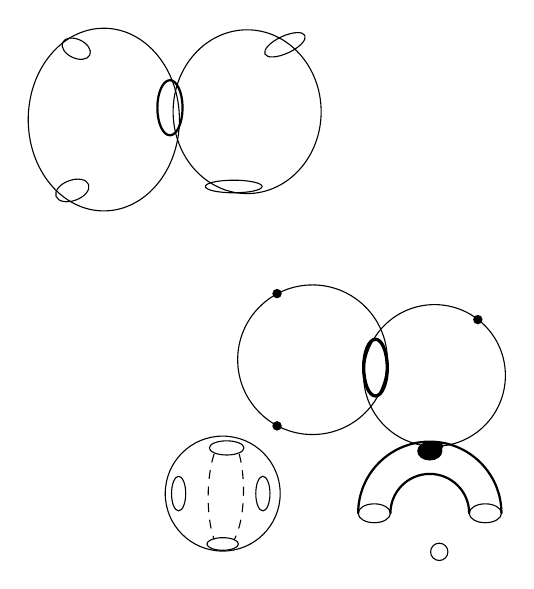
\begin{tikzpicture}[x=1mm,y=-1mm,line cap=round,line join=round,font=\small]
\draw (19,18.5) ellipse [x radius=9.6, y radius=11.6];
\draw (37.2,17.5) ellipse [x radius=9.4, y radius=10.4];
\draw[rotate around={-25:(15.5,9.5)}] (15.5,9.5) ellipse [x radius=1.9, y radius=1.2];
\draw[rotate around={20:(15,27.5)}] (15,27.5) ellipse [x radius=2.2, y radius=1.3];
\draw[thick] (27.4,17) ellipse [x radius=1.6, y radius=3.5];
\draw[rotate around={25:(42,9)}] (42,9) ellipse [x radius=2.8, y radius=1.1];
\draw (35.5,27) ellipse [x radius=3.6, y radius=0.8];
\draw (45.5,49) circle [radius=9.5];
\draw (61,51) circle [radius=9];
\draw[very thick] (53.5,50) ellipse [x radius=1.5, y radius=3.6];
\fill (41,40.6) circle [radius=0.6];
\fill (41,57.4) circle [radius=0.6];
\fill (66.5,43.9) circle [radius=0.6];
\fill (61.5,60) circle [radius=0.6];
\draw (34.1,66) circle [radius=7.3];
\draw (28.5,66) ellipse [x radius=0.9, y radius=2.2];
\draw (39.2,66) ellipse [x radius=0.9, y radius=2.2];
\draw (34.6,60.2) ellipse [x radius=2.2, y radius=0.9];
\draw (34.1,72.4) ellipse [x radius=2, y radius=0.8];
\draw[dashed] (33,61) .. controls (32,64) and (32,69) .. (33,71.8);
\draw[dashed] (36.2,61) .. controls (37,64) and (37,69) .. (35.6,71.8);
\draw[thick] (51.3,68.5) arc [start angle=180, end angle=360, radius=9.1];
\draw[thick] (55.4,68.5) arc [start angle=180, end angle=360, radius=5];
\draw (53.35,68.5) ellipse [x radius=2.05, y radius=1.2];
\draw (67.45,68.5) ellipse [x radius=2.05, y radius=1.2];
\fill (60.4,60.6) ellipse [x radius=1.6, y radius=1.2];
\draw (61.6,73.4) circle [radius=1.1];
\end{tikzpicture}
\end{document}
